\documentclass[11pt,a4paper]{article}
\usepackage[utf8]{inputenc}
\usepackage[T1]{fontenc}
\usepackage{amsmath,amssymb,amsfonts}
\usepackage{graphicx}
\usepackage{booktabs}
\usepackage{hyperref}
\usepackage{listings}
\usepackage{xcolor}
% Algorithm pseudocode via verbatim (avoiding algorithm package dependency)
\usepackage{tikz}
\usetikzlibrary{shapes,arrows,positioning,fit,backgrounds}
\usepackage{subcaption}
\usepackage{enumitem}
\usepackage[margin=1in]{geometry}

% Code listing style
\lstdefinestyle{json}{
    basicstyle=\ttfamily\small,
    keywordstyle=\color{blue},
    stringstyle=\color{red},
    commentstyle=\color{gray},
    breaklines=true,
    frame=single,
    showstringspaces=false
}

\lstdefinestyle{rego}{
    basicstyle=\ttfamily\small,
    keywordstyle=\color{purple},
    stringstyle=\color{orange},
    commentstyle=\color{gray},
    breaklines=true,
    frame=single,
    showstringspaces=false,
    morekeywords={package,import,deny,contains,if,some,in,input}
}

\title{\textbf{aflock: Cryptographically Signed Policies for\\Constrained AI Agent Execution}}

\author{
    Cole Kennedy\thanks{Corresponding author. Email: cole@testifysec.com} \\
    TestifySec, Inc.
}

\date{January 2026}

\begin{document}

\maketitle

\begin{abstract}
As AI agents become increasingly autonomous---executing commands, accessing APIs, spawning sub-agents, and managing sensitive data---ensuring they operate within authorized bounds becomes critical. We present \textbf{aflock}, a policy framework that cryptographically constrains AI agent behavior through signed policy files, verifiable attestations, and cross-step constraint verification. Unlike existing approaches that rely on runtime guardrails or trusted execution environments, aflock provides a software-only solution inspired by workload identity systems (SPIFFE/SPIRE) and software supply chain security (in-toto). Key innovations include: (1) agent identity derivation from introspectable properties (model, environment, tools) via MCP socket inspection, (2) separation of JWT-based authorization from server-held signing keys, (3) session merkle trees for ordering and completeness proofs, (4) sublayouts for hierarchical sub-agent delegation with attenuated constraints, and (5) cross-step Rego evaluation for cumulative limit enforcement. We position aflock within the emerging landscape of agent security frameworks and outline a verification algorithm that enables post-hoc compliance auditing with cryptographic guarantees.
\end{abstract}

\section{Introduction}

The proliferation of autonomous AI agents presents a fundamental security challenge: how do principals (humans, organizations, or parent agents) constrain what an agent can do, prove it operated within bounds, and verify compliance after the fact?

Consider a software development agent tasked with implementing a feature. It may read files, execute shell commands, make API calls, and even spawn sub-agents for research tasks. Without constraints, such an agent could:
\begin{itemize}[noitemsep]
    \item Exceed cost budgets through unbounded API usage
    \item Access sensitive files (credentials, environment variables)
    \item Execute dangerous commands (force pushes, destructive operations)
    \item Exfiltrate data through unrestricted network access
    \item Delegate unconstrained authority to sub-agents
\end{itemize}

Existing solutions address fragments of this problem. Runtime guardrails~\cite{guardrailsai} filter inputs and outputs but provide no cryptographic proof of compliance. Trusted execution environments~\cite{omega2025} offer strong isolation but require specialized hardware. Identity frameworks~\cite{spiffe} authenticate workloads but weren't designed for non-deterministic AI agents.

We present \textbf{aflock}, a policy framework that treats agent constraints like dependency locks treat package versions---as signed, immutable specifications that the agent cannot modify. The name derives from ``agent flow lock,'' analogous to how \texttt{package-lock.json} locks dependencies in software projects.

\subsection{Contributions}

This paper makes the following contributions:

\begin{enumerate}
    \item \textbf{Policy Schema}: A comprehensive JSON schema for expressing agent constraints including resource limits, tool allowlists, file access patterns, and evaluator specifications.

    \item \textbf{Identity Derivation}: A mechanism for deriving agent identity from introspectable properties (model, environment, tools, policy digest) via MCP socket inspection, inspired by SPIRE's workload attestation.

    \item \textbf{Attestation Model}: An in-toto-compatible attestation format for agent actions that enables cryptographic verification of constraint compliance.

    \item \textbf{Cross-Step Verification}: A Rego-based evaluation framework that accesses attestations across all execution steps for cumulative constraint checking.

    \item \textbf{Sublayout Delegation}: A hierarchical model for sub-agent policy delegation with mandatory constraint attenuation, inspired by in-toto sublayouts.
\end{enumerate}

\section{Threat Model and Assumptions}

\subsection{Threat Model}

We consider an adversarial agent that attempts to:
\begin{itemize}[noitemsep]
    \item \textbf{Exceed resource limits}: Consume more tokens, API calls, or cost than authorized
    \item \textbf{Access unauthorized resources}: Read/write files, call APIs, or access secrets outside the allowlist
    \item \textbf{Forge attestations}: Create false records of compliant behavior
    \item \textbf{Escalate privileges}: Spawn sub-agents with greater authority than the parent
    \item \textbf{Tamper with ordering}: Reorder, omit, or inject execution steps
\end{itemize}

\subsection{Trust Assumptions}

\begin{enumerate}
    \item \textbf{aflock server integrity}: The aflock server (analogous to a SPIRE server) is trusted and controls signing keys
    \item \textbf{Policy signer authenticity}: Policies are signed by authorized principals (humans or trusted systems)
    \item \textbf{Transport security}: MCP communication occurs over authenticated channels
    \item \textbf{Process isolation}: The OS enforces process boundaries (agents cannot inspect other processes' memory)
    \item \textbf{Tool-call mediation}: Agent actions are routed through aflock's MCP tool gate. Native subagent execution can bypass tool-level enforcement without a kernel sandbox.
\end{enumerate}

For stronger guarantees, run aflock inside a kernel-enforced sandbox (e.g., nono) so filesystem and network restrictions apply to all descendant processes.

We explicitly \textbf{do not} assume:
\begin{itemize}[noitemsep]
    \item Trusted execution environments (TEE)
    \item Hardware security modules (HSM)
    \item Deterministic agent behavior
    \item Agent honesty or cooperation
\end{itemize}

\section{System Architecture}

Figure~\ref{fig:architecture} illustrates the aflock architecture. The system consists of three primary components: the AI agent, the aflock server, and the verification layer.

\begin{figure}[t]
\centering
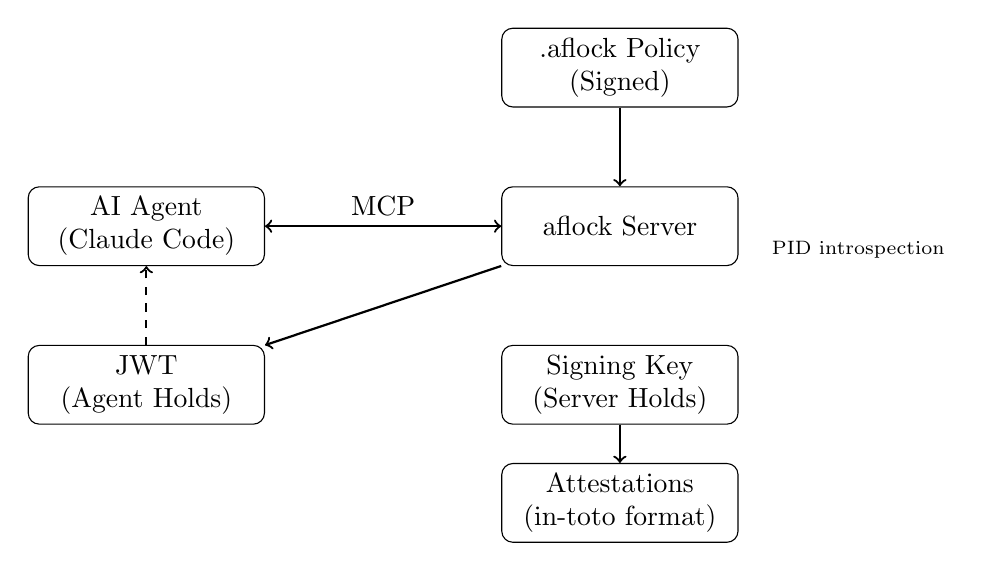
\begin{tikzpicture}[
    node distance=1.5cm,
    box/.style={rectangle, draw, rounded corners, minimum width=3cm, minimum height=1cm, align=center},
    arrow/.style={->, thick}
]
    % Agent
    \node[box] (agent) {AI Agent\\(Claude Code)};

    % aflock Server
    \node[box, right=3cm of agent] (server) {aflock Server};

    % Components below
    \node[box, below=1cm of agent] (jwt) {JWT\\(Agent Holds)};
    \node[box, below=1cm of server] (key) {Signing Key\\(Server Holds)};

    % Policy
    \node[box, above=1cm of server] (policy) {.aflock Policy\\(Signed)};

    % Attestations
    \node[box, below=2.5cm of server] (attest) {Attestations\\(in-toto format)};

    % Arrows
    \draw[arrow, <->] (agent) -- node[above] {MCP} (server);
    \draw[arrow] (server) -- (jwt);
    \draw[arrow] (policy) -- (server);
    \draw[arrow] (key) -- (attest);
    \draw[arrow, dashed] (jwt) -- (agent);

    % PID introspection
    \node[right=0.3cm of server, yshift=-0.3cm, font=\scriptsize] {PID introspection};

\end{tikzpicture}
\caption{aflock architecture showing separation between agent-held JWT and server-held signing key. The agent communicates via MCP; the server derives identity through PID introspection.}
\label{fig:architecture}
\end{figure}

\subsection{Agent Identity Derivation}

A core insight of aflock is that agent identity should be \textit{derived} from introspectable properties rather than \textit{assigned}. When an agent connects to the aflock server via MCP over a Unix domain socket, the server can obtain the connecting process's PID through \texttt{SO\_PEERCRED} (Linux) or \texttt{LOCAL\_PEERCRED} (macOS).

From the PID, the server introspects:
\begin{itemize}[noitemsep]
    \item \textbf{Binary path}: The executable running the agent
    \item \textbf{User/Group ID}: Process ownership
    \item \textbf{Container ID}: If running in a container (via \texttt{/proc/PID/cgroup})
    \item \textbf{Environment variables}: Model configuration, session identifiers
\end{itemize}

Combined with information from the MCP handshake (model name, available tools), the server computes:

\begin{equation}
\text{AgentIdentity} = \text{SHA256}(\text{model} \| \text{env} \| \text{tools} \| \text{policyDigest} \| \text{parent})
\end{equation}

This approach mirrors SPIRE's workload attestation~\cite{spiffe}, where identity emerges from verifiable properties rather than self-declaration. The agent \textit{cannot lie about its identity} because the server independently verifies all components.

\subsection{JWT and Signing Key Separation}

A critical security property is the separation between authorization (what the agent is allowed to do) and attestation (proof of what the agent did). The agent receives a short-lived JWT containing:

\begin{lstlisting}[style=json]
{
  "sub": "sha256:a1b2c3...",
  "iat": 1737200000,
  "exp": 1737203600,
  "grants": {
    "tools": ["Read", "Edit", "Bash"],
    "files": {"allow": ["src/**"], "deny": ["**/.env"]},
    "limits": {"maxSpendUSD": 10.00}
  }
}
\end{lstlisting}

The agent presents this JWT when requesting actions, but \textit{all attestations are signed by a key the agent never sees}. This ensures that even a compromised agent cannot forge attestations claiming compliant behavior.

\subsection{MCP Integration}

The Model Context Protocol (MCP) provides the communication channel between agent and server. The aflock server exposes MCP tools for:

\begin{itemize}[noitemsep]
    \item \texttt{aflock\_authorize}: Request authorization for an action
    \item \texttt{aflock\_attest}: Record an action (server signs attestation)
    \item \texttt{aflock\_check\_limits}: Query remaining budget
    \item \texttt{aflock\_delegate}: Create sublayout for sub-agent
\end{itemize}

This design allows aflock to integrate with any MCP-compatible agent (Claude Code, custom agents) without modification to the agent's core logic.

\section{Policy Schema}

The \texttt{.aflock} policy file is a signed JSON document specifying all constraints on agent behavior. We describe the key sections.

\subsection{Identity Constraints}

\begin{lstlisting}[style=json]
{
  "identity": {
    "allowedModels": ["claude-opus-4-5-20251101", "claude-sonnet-4-*"],
    "allowedEnvironments": ["container:ghcr.io/org/*", "user:deploy-*"],
    "requiredTools": ["Read", "Edit"]
  }
}
\end{lstlisting}

Identity constraints specify which agent configurations are authorized to operate under this policy. Glob patterns enable flexible matching while maintaining security.

\subsection{Resource Limits}

\begin{lstlisting}[style=json]
{
  "limits": {
    "maxSpendUSD": {"value": 10.00, "enforcement": "fail-fast"},
    "maxTokensIn": {"value": 500000, "enforcement": "fail-fast"},
    "maxTurns": {"value": 50, "enforcement": "post-hoc"},
    "maxWallTimeSeconds": {"value": 3600, "enforcement": "fail-fast"}
  }
}
\end{lstlisting}

Each limit specifies an enforcement mode:
\begin{itemize}[noitemsep]
    \item \textbf{fail-fast}: Abort immediately when breached (for cost, security)
    \item \textbf{post-hoc}: Verify at completion (for quality, turn count)
\end{itemize}

\subsection{Grants and Allowlists}

\begin{lstlisting}[style=json]
{
  "tools": {
    "allow": ["Read", "Edit", "Bash", "Glob", "Grep"],
    "deny": ["Task"],
    "requireApproval": ["Bash:rm -rf *", "Bash:git push --force"]
  },
  "files": {
    "allow": ["src/**", "tests/**"],
    "deny": ["**/.env", "**/secrets/**"],
    "readOnly": ["package.json", "go.mod"]
  },
  "grants": {
    "secrets": {"allow": ["vault:secret/data/readonly/*"]},
    "apis": {"allow": ["https://api.anthropic.com/*"]}
  }
}
\end{lstlisting}

The allowlist model follows the principle of least privilege: all access is denied unless explicitly granted.

\subsection{Materials Binding}

\begin{lstlisting}[style=json]
{
  "materialsFrom": {
    "session": {
      "path": "${CLAUDE_SESSION_PATH}",
      "algorithm": "sha256",
      "merkleTree": true
    },
    "git": {
      "treeHash": "${GIT_TREE_HASH}"
    }
  }
}
\end{lstlisting}

The \texttt{materialsFrom} directive binds the policy to external artifacts. The session merkle tree is particularly important: by constructing a merkle tree over the session JSONL, we can prove:
\begin{itemize}[noitemsep]
    \item \textbf{Order}: Turn $n$ came after turns $0$ through $n-1$
    \item \textbf{Completeness}: No turns were omitted
    \item \textbf{Distance}: Turns are contiguous (no gaps)
\end{itemize}

\subsection{Evaluators}

aflock supports two types of evaluators for constraint verification:

\subsubsection{Rego Evaluators}

\begin{lstlisting}[style=rego]
package aflock
import rego.v1

turns := [t | some t in input.attestations]
sum_spend := sum([t.predicate.metrics.costUSD | some t in turns])

deny contains msg if {
    sum_spend > input.policy.limits.maxSpendUSD.value
    msg := sprintf("Spend $%.2f exceeds $%.2f",
                   [sum_spend, input.policy.limits.maxSpendUSD.value])
}
\end{lstlisting}

Rego policies enable cross-step verification: the evaluator receives all attestations and can compute cumulative metrics.

\subsubsection{AI Evaluators}

\begin{lstlisting}[style=json]
{
  "evaluators": {
    "ai": [{
      "name": "quality-check",
      "prompt": "PASS if code is production-ready. FAIL otherwise.",
      "model": "claude-opus-4-5-20251101"
    }]
  }
}
\end{lstlisting}

AI evaluators assess qualitative properties that are difficult to express in formal logic, such as code quality or task completion.

\section{Sublayouts: Hierarchical Delegation}

Inspired by in-toto sublayouts~\cite{intoto}, aflock supports hierarchical sub-agent delegation with mandatory constraint attenuation.

\begin{lstlisting}[style=json]
{
  "sublayouts": [{
    "name": "research-agent",
    "policy": "./policies/research.aflock",
    "limits": {"maxSpendUSD": {"value": 2.00}},
    "inherit": ["domains", "functionaries"]
  }]
}
\end{lstlisting}

The following invariants are enforced:
\begin{enumerate}
    \item \textbf{Attenuation}: Sub-agent limits must be $\leq$ parent limits
    \item \textbf{Accumulation}: Sub-agent spend counts toward parent totals
    \item \textbf{Namespacing}: Sub-agent attestations are prefixed with sublayout name
    \item \textbf{Recursion}: Verification recurses into sublayouts
\end{enumerate}

\section{Verification Algorithm}

The verification procedure for an aflock-constrained execution proceeds in six phases:

\begin{figure}[t]
\begin{lstlisting}[basicstyle=\ttfamily\small,frame=single,caption={aflock Verification Algorithm},label={alg:verify}]
VERIFY(Policy P, Attestations A, Materials M):

  Phase 1: Signature Verification
    for each attestation a_i in A:
      if not VerifySignature(a_i, P.functionaries):
        return FAIL: "Invalid signature on attestation i"

  Phase 2: Identity Verification
    for each attestation a_i in A:
      if not MatchesIdentity(a_i.agent, P.identity):
        return FAIL: "Identity mismatch on attestation i"

  Phase 3: Materials Binding
    if P.materialsFrom.session.merkleTree:
      root = ComputeMerkleRoot(M.session)
      if root != A[n].predicate.sessionRoot:
        return FAIL: "Session merkle root mismatch"

  Phase 4: Constraint Evaluation
    for each Rego evaluator e in P.evaluators.rego:
      result = EvaluateRego(e.policy, {P, A, M})
      if result.deny is not empty:
        return FAIL: result.deny

  Phase 5: AI Evaluation
    for each AI evaluator e in P.evaluators.ai:
      result = EvaluateAI(e.prompt, e.model, M)
      if result == FAIL:
        return FAIL: "AI evaluator 'e.name' failed"

  Phase 6: Sublayout Recursion
    for each sublayout s in P.sublayouts:
      A_s = {a in A : a.prefix == s.name}
      result = VERIFY(s.policy, A_s, M)
      if result == FAIL:
        return FAIL: "Sublayout 's.name' failed"

  return PASS
\end{lstlisting}
\end{figure}

\section{Related Work}

Table~\ref{tab:comparison} compares aflock to related systems across key capabilities.

\begin{table}[t]
\centering
\caption{Comparison of AI agent constraint systems}
\label{tab:comparison}
\begin{tabular}{lccccc}
\toprule
\textbf{Capability} & \textbf{Omega} & \textbf{VeriGuard} & \textbf{ARIA} & \textbf{ShieldAgent} & \textbf{aflock} \\
\midrule
Signed policy file & ? & \texttimes & \texttimes & \texttimes & \checkmark \\
Identity derivation & TEE & \texttimes & DID & \texttimes & PID+MCP \\
Cryptographic attestations & \checkmark & \texttimes & VC & \texttimes & in-toto \\
Cross-step verification & ? & \texttimes & \texttimes & \texttimes & Rego \\
Spend/token limits & \texttimes & \texttimes & \texttimes & \texttimes & \checkmark \\
Sub-agent delegation & ? & \texttimes & \checkmark & \texttimes & sublayouts \\
Session ordering proofs & \texttimes & \texttimes & \texttimes & \texttimes & Merkle \\
Software-only (no TEE) & \texttimes & \checkmark & \checkmark & \checkmark & \checkmark \\
\bottomrule
\end{tabular}
\end{table}

\subsection{Trusted Execution Approaches}

Omega~\cite{omega2025} provides strong isolation guarantees through confidential VMs and GPUs (AMD SEV-SNP, NVIDIA H100). While offering hardware-backed security, this approach requires specialized infrastructure unavailable in many deployment contexts. aflock provides a software-only alternative with cryptographic (rather than hardware) guarantees.

\subsection{Formal Verification}

VeriGuard~\cite{veriguard2025} applies formal verification to agent policies using Hoare triples, proving safety properties before execution. This approach complements aflock: VeriGuard could verify policy correctness while aflock provides runtime attestation that the policy was followed.

\subsection{Identity Frameworks}

SPIFFE/SPIRE~\cite{spiffe} provides the architectural inspiration for aflock's identity derivation. However, SPIFFE treats workload replicas as identical---appropriate for deterministic microservices but problematic for non-deterministic AI agents. aflock extends this model with policy-aware identity binding.

ARIA~\cite{aria2025} proposes a graph-native identity model with DIDs and verifiable credentials. While powerful for complex delegation scenarios, ARIA's graph-based approach adds complexity that may be unnecessary for simpler agent deployments.

\subsection{Runtime Guardrails}

ShieldAgent~\cite{shieldagent2025} and AgentGuardian~\cite{agentguardian2026} provide runtime policy enforcement but lack cryptographic attestation. These systems cannot prove compliance after the fact---a critical requirement for regulated industries.

\subsection{Token-Based Delegation}

Google's Macaroons~\cite{macaroons} and Biscuit tokens~\cite{biscuit} provide elegant primitives for offline attenuation and delegation. aflock could adopt these as transport mechanisms while providing the higher-level policy semantics and attestation framework.

\subsection{Cost Management}

Google's Budget Tracker~\cite{budgettracker2025} injects budget awareness into agent reasoning loops. aflock's limit enforcement provides similar functionality with the addition of cryptographic proof that limits were respected.

\section{Discussion}

\subsection{Limitations}

\textbf{Trust in aflock server}: The aflock server holds signing keys and must be trusted. A compromised server could forge attestations. Mitigations include HSM-backed keys and multi-party signing.

\textbf{MCP dependency}: aflock requires MCP-compatible agents. Agents using other protocols require adapters.

\textbf{AI evaluator reliability}: AI-based quality checks are probabilistic. Critical constraints should use Rego policies for deterministic verification.

\textbf{Performance overhead}: Attestation signing adds latency to each action. Batching strategies can mitigate this for high-frequency operations.

\subsection{Future Work}

\textbf{Distributed verification}: Enabling third parties to verify attestations without accessing the full execution trace.

\textbf{Policy inheritance}: Allowing policies to extend base templates for organizational standardization.

\textbf{Real-time monitoring}: Streaming attestations to monitoring systems for live compliance dashboards.

\textbf{Formal semantics}: Developing a formal semantics for the policy language to enable policy analysis and composition verification.

\section{Conclusion}

aflock provides a comprehensive framework for constraining AI agent behavior through cryptographically signed policies and verifiable attestations. By combining insights from workload identity (SPIFFE/SPIRE), software supply chain security (in-toto), and capability-based authorization (Macaroons), aflock enables principals to define, enforce, and verify agent constraints without requiring trusted hardware.

As AI agents become more autonomous and widely deployed, frameworks like aflock will be essential for maintaining human oversight and regulatory compliance. The separation of authorization (JWT) from attestation (server-signed) ensures that even compromised agents cannot forge evidence of compliant behavior.

We release the aflock specification and examples at \url{https://github.com/aflock-ai/aflock} to enable community feedback and adoption.

\bibliographystyle{plain}
\begin{thebibliography}{10}

\bibitem{omega2025}
Author et al.
\newblock Omega: Trusted AI Agents in the Cloud.
\newblock {\em arXiv preprint arXiv:2512.05951}, 2025.

\bibitem{veriguard2025}
Lesly Miculicich et al.
\newblock VeriGuard: Enhancing LLM Agent Safety via Verified Code Generation.
\newblock {\em arXiv preprint arXiv:2510.05156}, 2025.

\bibitem{shieldagent2025}
Zhaorun Chen, Mintong Kang, Bo Li et al.
\newblock ShieldAgent: Shielding Agents via Verifiable Safety Policy Reasoning.
\newblock {\em arXiv preprint arXiv:2503.22738}, 2025.

\bibitem{agentguardian2026}
Nadya Abaev, Denis Klimov et al.
\newblock AgentGuardian: Learning Access Control Policies to Govern AI Agent Behavior.
\newblock {\em arXiv preprint arXiv:2601.10440}, 2026.

\bibitem{spiffe}
CNCF.
\newblock SPIFFE: Secure Production Identity Framework For Everyone.
\newblock \url{https://spiffe.io/}, 2024.

\bibitem{intoto}
Santiago Torres-Arias et al.
\newblock in-toto: Providing farm-to-table guarantees for bits and bytes.
\newblock In {\em USENIX Security Symposium}, 2019.

\bibitem{macaroons}
Arnar Birgisson et al.
\newblock Macaroons: Cookies with Contextual Caveats for Decentralized Authorization in the Cloud.
\newblock In {\em Network and Distributed System Security Symposium (NDSS)}, 2014.

\bibitem{biscuit}
Geoffroy Couprie.
\newblock Biscuit: Authorization tokens with decentralized verification.
\newblock \url{https://www.biscuitsec.org/}, 2024.

\bibitem{aria2025}
ISACA.
\newblock The Looming Authorization Crisis: Why Traditional IAM Fails Agentic AI.
\newblock {\em ISACA Industry News}, 2025.

\bibitem{guardrailsai}
Guardrails AI.
\newblock Guardrails: Adding guardrails to large language models.
\newblock \url{https://www.guardrailsai.com/}, 2024.

\bibitem{budgettracker2025}
Google Research.
\newblock Budget Tracker and BATS Framework for AI Agent Cost Control.
\newblock {\em Google AI Blog}, 2025.

\end{thebibliography}

\appendix

\section{Full Policy Schema}
\label{appendix:schema}

The complete JSON Schema for \texttt{.aflock} files is available at:
\url{https://github.com/aflock-ai/aflock/blob/main/docs/spec.md}

\section{Example: Compliance Control Evaluation}

\begin{lstlisting}[style=json,caption={OSCAL compliance evaluation policy}]
{
  "version": "1.0",
  "name": "oscal-control-evaluation",
  "expires": "2026-06-01T00:00:00Z",

  "identity": {
    "allowedModels": ["claude-opus-4-5-*"],
    "allowedEnvironments": ["container:ghcr.io/testifysec/*"]
  },

  "limits": {
    "maxSpendUSD": {"value": 25.00, "enforcement": "fail-fast"},
    "maxTokensIn": {"value": 1000000, "enforcement": "post-hoc"}
  },

  "tools": {
    "allow": ["Read", "Write", "Glob", "Grep", "Bash", "WebFetch"],
    "deny": ["Task"]
  },

  "evaluators": {
    "rego": [{
      "name": "all-controls-assessed",
      "policy": "deny contains msg if { count(missing_controls) > 0 }"
    }],
    "ai": [{
      "name": "assessment-quality",
      "prompt": "PASS if each control assessment includes evidence references and remediation guidance. FAIL otherwise.",
      "model": "claude-opus-4-5-20251101"
    }]
  },

  "sublayouts": [{
    "name": "evidence-collector",
    "policy": "./policies/evidence.aflock",
    "limits": {"maxSpendUSD": {"value": 5.00}}
  }]
}
\end{lstlisting}

\end{document}
